\documentclass{article}
\usepackage{amsmath}
\usepackage{amsfonts}
\usepackage{array}
\usepackage{dsfont}
\usepackage{hyperref}
\usepackage{amssymb}
\usepackage{amsthm}
\usepackage{amsfonts}
\usepackage{graphicx}
% \usepackage{geometry}
\usepackage{bbold}
\usepackage{caption}
% \usepackage{pseudocode}
\usepackage{standalone}
% \usepackage[nottoc]{tocbibind}
% \usepackage{apacite}
\usepackage{etoolbox}
% \usepackage{tikz}
% \usepackage{color}
% \usepackage[T1]{fontenc}
% \usepackage{lmodern}
% \usepackage{mathptmx}
% \usepackage{standalone}
\usepackage{accents}
\usepackage{enumitem}

% used for typesetting theorem environments
\usepackage{amsthm}

% used for typesetting tikz graphs
\usepackage{tikz}
% used for typesetting automata using tikz
\usetikzlibrary{automata}


% aaron edit

%wills stuff


\usepackage{tikz}
\usepackage{algorithmic}
\usepackage{algorithm}
\usepackage{verbatim}
\usepackage[super]{nth}

\graphicspath{ {images/} }

\newcommand{\R}{\mathds{R}}
\newcommand{\Zplus}{\mathds{Z}_+}
\newcommand{\N}{\mathds{N}}
\newcommand{\seq}[2][j]{\left\{#2\right\}_{#1=0}^\infty}
\newcommand{\diff}[3][]{\frac{\mathrm{d}^{#1} #2}{\mathrm{d}^{#1} #3}}
\newcommand{\pdiff}[3][]{\frac{\partial^{#1} #2}{\partial^{#1} #3}}
\newcommand{\dd}{\mathrm{d}}
\newcommand{\ip}[2]{\left\langle #1,#2\right\rangle}
\newcommand{\kernl}[1]{\text{ker}(#1)}
\newcommand{\ind}[1]{\mathbb{1}_{#1}~}
\newcommand{\s}{\mathcal{S}}
\newcommand{\Sin}[1]{\sin\left(#1\right)}
\newcommand{\Cos}[1]{\cos\left(#1\right)}
\newcommand{\ubar}[1]{\underaccent{\bar}{#1}}
\newcommand{\argmin}[1]{\underset{#1}{\operatorname{argmin}}\;}

\newtheorem{thm}{Theorem}
\newtheorem{assmp}{Assumption}
\newtheorem{prop}{Proposition}
\newtheorem{lemma}{Lemma}

\newcolumntype{C}[1]{>{\centering\arraybackslash}p{#1}}
\newcolumntype{L}[1]{>{\raggedright\arraybackslash}p{#1}}
\newcolumntype{R}[1]{>{\raggedleft\arraybackslash}p{#1}}

\captionsetup[table]{labelfont=bf}
\captionsetup[figure]{labelfont=bf}

\title{Group 5 Thesis}
\author{Us}

\begin{document}
	\maketitle

	\section{Introduction}
		Imagine an object recorded by a camera and represented in a sequence of 2-dimensional, coloured images. The object may change size due to changes in position (closer to the camera) or even by nature (an inflating balloon). The object may enter a shadow or areas with different lighting causing its brightness and colour to change between images. If the object or the camera moves and rotates, then the location of the object, its shape, and even the background of the object will alter over the sequence of images. Nonetheless, a human could view this sequence of images and associate a region in each image as one object being manipulated. 

		Region tracking in a sequence of images seeks to create a computer program that, given a region in an initial image, can identify the region over subsequent images. The tracking is desired to be achieved even if some characteristics of the region change. This report proposes two distinct applications for such a program: hand-gesture tracking and tracking of anatomical structures of CT/MRI scans. While hand-gesture recognition will process images whose sequence represents change in time, the CT/MRI scan will process images whose sequence represents change along a dimension of the 3-dimensional object that was scanned.

<<<<<<< HEAD
		\subsection{Application: Medical Imaging}
			The main imaging modalities chosen were X-ray Computed Tomography (CT) and Magnetic Resonance Imaging (MRI) scans. These modalities were chosen due to their diagnostic performance and ubiquity of use. For surgeons these scans are an integral portion of planning and preparing for procedures. The ability to automatically segment tissues and render models of them in 3D aids in this process and can also be used to produce implants that fit the patient's anatomy to a greater degree.


		\subsection{Application: Gesture Tracking}
			Following a hand through a video sequence can provide individuals with a touchless interface like the Kinect. Using the cheap an ubiquitous web cam the ability to follow gestures can allow a user to interact more fluidly with technology and prevent interruption of some tasks.
=======
		\subsection{Appliction: Medical Imaging}
			The main imaging modalities chosen were X-ray Computed Tomography (CT) and Magtetic Resinance Imaging (MRI) scans. These modalities were chosen due to their diagnostic proformance and ubiqity of use. For surgons these scans are an integral portion of planning and preparing for precedures. The ability to automaticaly segment tissues and render models of them in 3D aids in this process and can also be used to produce implants that fit the pateint's antomy to a greater degrree.


		\subsection{Aplication: Gesture Tracking}
			Following a hand through a video sequence can provide individual with a touchless interface like the Kinect. Using the cheap an ubiqitus web cam the ability to follow gestures can allow a user to interact more fluidly with technology and prevent interuption of some tasks.
>>>>>>> 1cc6a8332fbe59243179d3490bb58a38f80979d9

	\section{Prob Def}
		Produce an algorithm that efficiently tracks regions in medical and video sequences with low error.

	\section{Math}
		\subsection{Problem Formulation}
			One of the most important design choices is the initial framing and structureing of the problem. By applying a riggerous mathimatical model to the design problem, a rich body of theory and tools were able to be used and implemented. The framework chosen was that of calculus of variation. This construction ultimatly turns the the problem of region tracking into a funtional minimization problem with convergance garenties. 

			To veiw region tracking under the the light of calculus of variation, some deffintions are needed first. let $\Omega = [0.1] \times [0,1]$ and let every image $I_i$ in the sequence $i\in \{1, 2, ... ,n\}$ be a mapping $\Omega \rightarrow \mathds{R}$. A region $R_i \subset \Omega$ is an element of $2^\Omega$ the power set of $\Omega$. The problem is now structured as finding $R_{l+1}$ given $I_l$, $I_{l+1}$ and $R_l$. To make this problem a functional minimization task, let $E:2^\Omega \rightarrow \mathds{R}$ such that $R_{l+1}$ is the minimizer of $E$.

			\subsection{Mathematical Tools}
				\subsubsection{Euler-Lagrange Necessary Conditions}
					The machinery of calculus of variation bestows the ability to potentially find a minimizer $\gamma^* = \argmin{\gamma \in C}E[\gamma]$. let $C$ be the set of simple closed curves defined as:
					\begin{center}
						$C = \{\gamma: [0,1]\rightarrow\R | \gamma \in \textbf{C}^2, \gamma(0)=\gamma(1),\dot\gamma(0)=\dot\gamma(1)\}$
					\end{center}
					Now define $E$ as a mapping $C\rightarrow\R$ and express it in the form of:
					\begin{equation} \label{eq:einlaform}
						E[\gamma] = \int_0^1{L(s,\gamma(s),\dot\gamma(s))ds}
					\end{equation}
					From optimization it is clear that the first order condition must be satisfied for an $x$ to be the minimizer of some function $f:\R^n\rightarrow\R$. The Euler-Lagrange necessary conditions are the functional analysis equivalent.

					\begin{thm} \label{th:el}
						Let $\gamma \in C$ be a minimizer of $E$ in the form of equation \ref{eq:einlaform} then $\forall s \in [0,1]$:
						\begin{equation} \label{eq:eleq}
							0 = \frac{\partial L}{\partial \gamma}\biggr\rvert_{(s,\gamma(s),\dot\gamma(s))}-\frac{d}{ds}\Bigg(\frac{\partial L}{\partial \dot\gamma}\biggr\rvert_{(s,\gamma(s),\dot\gamma(s))}\Bigg)
						\end{equation}
					\end{thm}
					
					\begin{proof}
						let $\phi$ be an element of $C$ and $\alpha\in\R$. As $\gamma$ is the minimizer of $E$ (implying $E(\gamma)\leq E(\theta)$ $\forall \theta\in C$), clearly $\frac{d}{d\alpha}E[\gamma + \alpha\phi]\rvert_{\alpha=0}=0$.

						\begin{align*}
							0 &= \frac{d}{d\alpha}E[\gamma + \alpha\phi]\rvert_{\alpha=0}\\
							&= \frac{d}{d\alpha}\int_0^1{L(s,\gamma(s) + \alpha\phi(s),\dot\gamma(s)+\alpha\dot\phi(s))ds}\biggr\rvert_{\alpha=0}\\
							&= \int_0^1{\frac{d}{d\alpha}L(s,\gamma(s) + \alpha\phi(s),\dot\gamma(s)+\alpha\dot\phi(s))\biggr\rvert_{\alpha=0}ds}\\
							&= \int_0^1{\frac{\partial L}{\partial \gamma}\biggr\rvert_{(s,\gamma(s),\dot\gamma(s))}\phi(s) + \frac{\partial L}{\partial \dot\gamma}\biggr\rvert_{(s,\gamma(s),\dot\gamma(s))}\dot\phi(s)ds}\\
							&= \int_0^1{\frac{\partial L}{\partial \gamma}\biggr\rvert_{(s,\gamma(s),\dot\gamma(s))}\phi(s)ds}+\int_0^1{\frac{\partial L}{\partial \dot\gamma}\biggr\rvert_{(s,\gamma(s),\dot\gamma(s))}\dot\phi(s)ds}\\
							&= \int_0^1{\frac{\partial L}{\partial \gamma}\biggr\rvert_{(s,\gamma(s),\dot\gamma(s))}\phi(s)ds} + \bigg[\frac{\partial L}{\partial \dot\gamma}\biggr\rvert_{(s,\gamma(s),\dot\gamma(s))}\phi(s)\bigg]_0^1 - \int_0^1{\frac{d}{ds}\bigg(\frac{\partial L}{\partial \dot\gamma}\biggr\rvert_{(s,\gamma(s),\dot\gamma(s))}\bigg)\phi(s)ds}\\
							&= \int_0^1{\frac{\partial L}{\partial \gamma}\biggr\rvert_{(s,\gamma(s),\dot\gamma(s))}\phi(s)ds} - \int_0^1{\frac{d}{ds}\bigg(\frac{\partial L}{\partial \dot\gamma}\biggr\rvert_{(s,\gamma(s),\dot\gamma(s))}\bigg)\phi(s)ds}\\
							&= \int_0^1{\bigg(\frac{\partial L}{\partial \gamma}\biggr\rvert_{(s,\gamma(s),\dot\gamma(s))} - \frac{d}{ds}\bigg(\frac{\partial L}{\partial \dot\gamma}\biggr\rvert_{(s,\gamma(s),\dot\gamma(s))}\bigg)\bigg)\phi(s)ds}\\
							&\Rightarrow 0 = \frac{\partial L}{\partial \gamma}\biggr\rvert_{(s,\gamma(s),\dot\gamma(s))} - \frac{d}{ds}\bigg(\frac{\partial L}{\partial \dot\gamma}\biggr\rvert_{(s,\gamma(s),\dot\gamma(s))}\bigg)
						\end{align*}
						The right hand side of equation \ref{eq:eleq} is continuous and the theorem thus holds for any choice of $\phi$.

					\end{proof}

					The techniques and tools employed in the Euler-Lagrange necessary condition proof provide a viable analogue to the the classic $\R^n$ gradient. Though theorem \ref{th:el} is a powerful result, it is only a necessary condition on the minimum and does not provide a method to find $\gamma^*$.

				\subsubsection{Gradient Decent}	
					Gradient Decent is one tool that has the ability to find critical points of the functional. To begin the $\R^n$ gradient decent schema will be illustrated then extended to the $C$-functional gradient decent system. 

					\begin{thm}\label{th:graddissimp}
						Let $f: \R^n\rightarrow\R$ such that $f$ is differentiable. Let $\nu$ be a mapping $\R^+ \rightarrow \R^n$ defined by:
						\begin{equation}\label{eq:decentsimp}
							\frac{d\nu(x)}{dt}(t) = -\vec\nabla f(\nu(t))
						\end{equation} 
						Then $f(\nu(t))$ is a monotonically decreasing function $\forall t\in\R^+$.
					\end{thm}
					\begin{proof}
						\begin{align*}
							\frac{d}{dt}f(\nu(t)) &= \langle \vec\nabla f(\nu(t)) , \frac{d}{dt}\nu(t)\rangle\\
							&= \langle \vec\nabla f(\nu(t)) , -\vec\nabla f(\nu(t))\rangle\\
							&= -\langle \vec\nabla f(\nu(t)) , \vec\nabla f(\nu(t))\rangle\\
							&= - \|\vec\nabla f(\nu(t))\|^2\\
							&\leq 0\\
						\end{align*}
						thus $f(\nu(t))$ is monotonically decreasing $\forall t\in\R^+$; with equality only at critical points of $f$.
					\end{proof}	

					Clearly by following this ordinary differential equation \ref{eq:decentsimp}, it is guaranteed that the system approaches a minimum or critical point.

					To extend these results to functionals, first define the set of evolving simple closed curves.

					\begin{equation}\label{eq:simpevolvecurv}
						C_e = \{\gamma: [0,1]\times\R^+\rightarrow\R | \gamma \in \textbf{C}^2, \gamma(0,t)=\gamma(1,t), \dot\gamma(0,t)=\dot\gamma(1,t),t\in\R^+\}
					\end{equation}

					\begin{thm}\label{th:decentfunc}
						Let $E$ be functional mapping $C$ to $\R$ and let $\gamma$ be an element of $C_e$ such that:
						\begin{equation}\label{eq:decentsimp}
							\frac{d\gamma}{dt}\biggr\rvert_{(s,t)} = - \Bigg(\frac{\partial L}{\partial \gamma}\biggr\rvert_{(s,\gamma(s,t),\dot\gamma(s,t))} - \frac{d}{ds}\bigg(\frac{\partial L}{\partial \dot\gamma}\biggr\rvert_{(s,\gamma(s,t),\dot\gamma(s,t))}\bigg)\Bigg)
						\end{equation} 
						Then $E(\gamma(t))$ is a monotonically decreasing function $\forall t\in\R^+$.
					\end{thm}

					\begin{proof}
						\begin{align*}
							\frac{d}{dt}E[\gamma(\cdot,t)] &= \frac{d}{dt}\int_0^1{L(s,\gamma(s,t),\dot\gamma(s,t))ds}\\
							&= \int_0^1{\frac{d}{dt}L(s,\gamma(s,t),\dot\gamma(s,t))ds}\\
							&= \int_0^1{\frac{\partial L}{\partial \gamma}\frac{\partial\gamma}{\partial t} + \frac{\partial L}{\partial \dot\gamma}\frac{\partial\dot\gamma}{\partial t}ds}\\
							&= \int_0^1{\frac{\partial L}{\partial \gamma}\frac{\partial\gamma}{\partial t} + \frac{\partial L}{\partial \dot\gamma}\frac{\partial^2\gamma}{\partial s\partial t}ds}\\
							&= \int_0^1{\frac{\partial L}{\partial \gamma}\frac{\partial\gamma}{\partial t} ds} + \bigg[\frac{\partial L}{\partial \dot\gamma}\frac{\partial\gamma}{\partial t}\bigg]_0^1 -\int_0^1{\frac{d}{ds}\bigg(\frac{\partial L}{\partial \dot\gamma}\frac{\partial\gamma}{\partial t}\bigg)ds}\\
							&= \int_0^1{\Bigg(\frac{\partial L}{\partial \gamma} - \frac{d}{ds}\bigg(\frac{\partial L}{\partial \dot\gamma}\bigg)\Bigg)\frac{\partial\gamma}{\partial t}ds}\\
							&= \int_0^1{\Bigg(\frac{\partial L}{\partial \gamma} - \frac{d}{ds}\bigg(\frac{\partial L}{\partial \dot\gamma}\bigg)\Bigg)^2 ds}\\
							&\leq 0
						\end{align*}
						Then $E(\gamma(t))$ is a monotonically decreasing function $\forall t\in\R^+$.
					\end{proof}
					These tools are now sufficient to begin designing and implementing an engineering solution to the problem.

		\subsection{Functionals}
			Give that $2^\Omega$ is a difficult set to work with and regions tend to consist of contiguous sections of $\omega$, it is reasonable to restrict regions to be those outlined by simple closed curves $\gamma$. This restriction opens up the powerful toolbox of calculus of variation. Within this framework gradient decent can be employed to numerically move towards the minima of the functionals $E$. Under this structure multiple functionals $E$ were designed for specific assumptions on the region characteristics.


			\subsubsection{The Length Functional}
				Under the assumption that that the region has "smooth" boundaries penalizing length of the curve is beneficial. 
				\begin{center}
					$E_L(\gamma) = \int_{0}^1{\|\dot\gamma(s)\|ds}$
				\end{center}

			\subsubsection{The $N^{th}$ Moment Functional}
				By assuming the distribution of gray scale within the image is conserved between regions the moment functional was devised. this functional ensures the $N^{th}$ moment is the same between regions and thus as the number of momnets used the distribution is conserved between the two.
				\begin{center}
				$E_{nM}(\gamma) = \Bigg(\frac{\int_{R_\gamma}{I_{l+1}(x)^n dx}}{\int_{R_\gamma}{dx}} - a\Bigg)^2 + \Bigg(\frac{\int_{R^{c}_\gamma}{I_{l+1}(x)^n dx}}{\int_{R^{c}_\gamma}{dx}} - b\Bigg)^2$ 
				\end{center}
			\subsubsection{The Center of Mass Functional}
				Many regions maintain a similar position in the image but may deform in space. By assuming relativity constant center of mass this trait is built int the functional.
				\begin{center}
					$E_{CM}(\gamma) = \Bigg(\frac{\int_{R_\gamma}{x dx}}{\int_{R_\gamma}{dx}} - a\Bigg)^2$ 
				\end{center}

			\subsubsection{The Area Functional}
				the last static property that was assumed was that area of the region is the same between images.
				\begin{center}
					$E_{A}(\gamma) = (\int_{R_\gamma}{dx} - a)^2$
				\end{center}

		\subsection{Level Sets}
			Though simple closed curves are  very intuitive to use, in practice their discretization and their instability for numerical gradient decent make them impractical. Level sets of of a function $u:\Omega\rightarrow\R$ can be used to define the region. In this technique the region $R_1 = {x: x\in\Omega|u(x)\geq0}$. Through the use of Green's Theorem it is possible to convert from a simple closed curve perspective to a level set perspective.

			

<<<<<<< HEAD
		\subsection{Functional Derivations} \label{sec:funcderiv}
=======
>>>>>>> 1cc6a8332fbe59243179d3490bb58a38f80979d9

	\section{Design}
	The functional pieces described in Section \ref{sec:funcderiv} had to be combined to form complete functionals. These functionals were created based on the invariant properties of the image sets. Of course, medical images and webcam-captured hand gesture images emphasize different invariant properties, thus functionals with different weighting on the functional pieces had to be designed for each application domain.

		\subsection{Medical Images}
		On the medical imaging side of the design, our project focused on high-contrast medical images such as those created by CT scans of bone. On these types of images, we were able to exploit high colour invariance of both the inside and outside of the outlined structure. To capture the colour properties of the images, we needed to heavily weigh inside and outside mean colour. Additionally, we also included the variance property in our functional, although this was weighted to a much weaker extent. The mean colour functional component captured the fact that the average colour on the inside and outside stayed relatively constant between images. The colour variance functional component captured a higher order term for the distribution of the pixel colours. On top of the mean and variance functionals, the length functional was added to stabilize the gradient descent.



		\subsection{Webcam-Generated Hand Gesture Images}
			Faisal

	\section{Implementation}
		Zach

	\section{Results}
		
		\subsection{Final Performance on Medical Images}
		The results of the algorithm using the final optimized parameters are shown in Figures \ref{fig:hip4_25}, \ref{fig:hip4_350}, and \ref{fig:hip4_375}. 
		\begin{figure}[H]
			\centering
			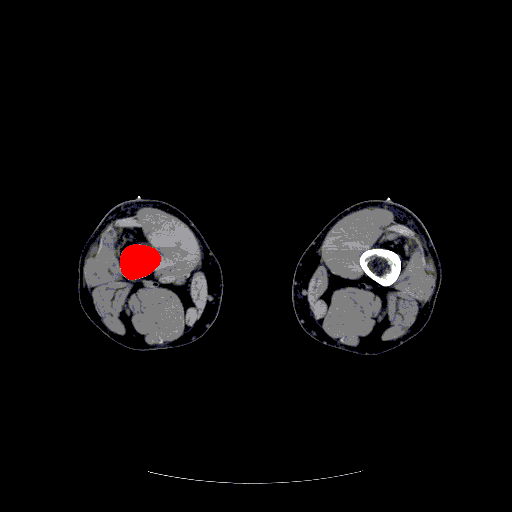
\includegraphics[width=0.4\textwidth]{Hip4/groundTruth25col.png}
			\hspace{20pt}
			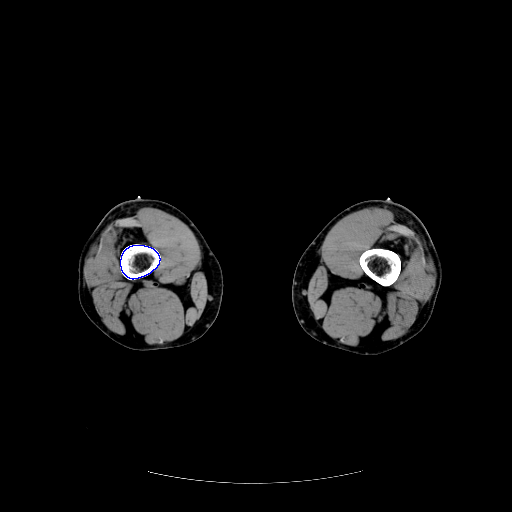
\includegraphics[width=0.4\textwidth]{Hip4/output25.png}
			\caption{Hip image 25 -- ground truth (left) compared to algorithm output with final parameter set (right).}
			\label{fig:hip4_25}
		\end{figure}
		\begin{figure}[H]
			\centering
			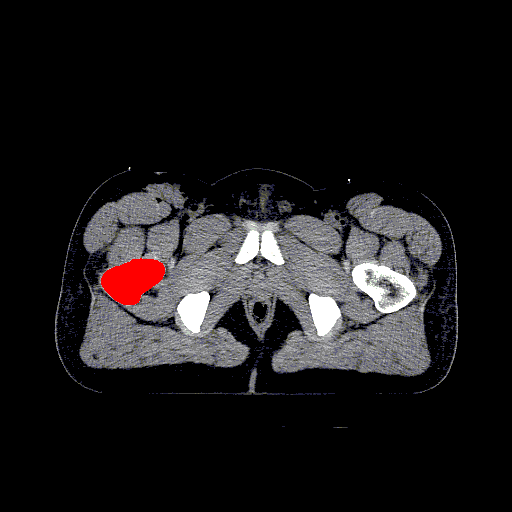
\includegraphics[width=0.4\textwidth]{Hip4/groundTruth350col.png}
			\hspace{20pt}
			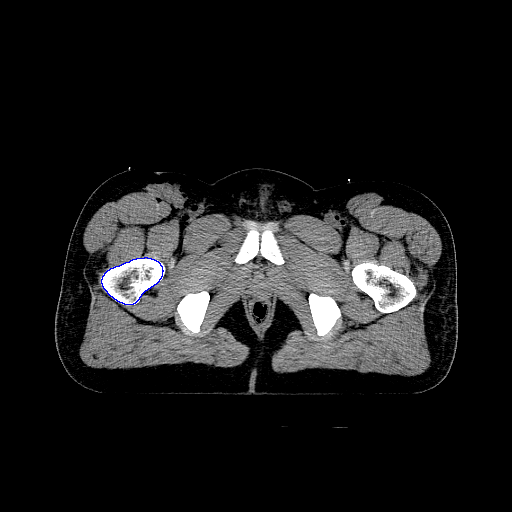
\includegraphics[width=0.4\textwidth]{Hip4/output350.png}
			\caption{Hip image 350 -- ground truth (left) compared to algorithm output with final parameter set (right).}
			\label{fig:hip4_350}
		\end{figure}
		\begin{figure}[H]
			\centering
			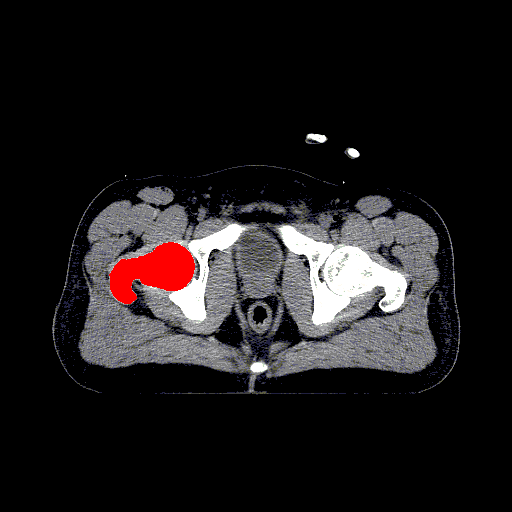
\includegraphics[width=0.4\textwidth]{Hip4/groundTruth375col.png}
			\hspace{20pt}
			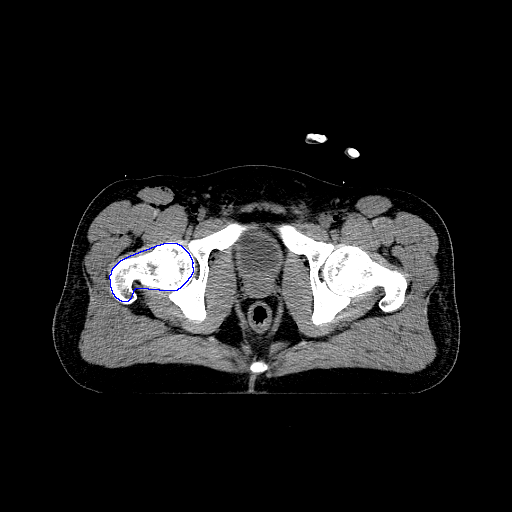
\includegraphics[width=0.4\textwidth]{Hip4/output375.png}
			\caption{Hip image 375 -- ground truth (left) compared to algorithm output with final parameter set (right).}
			\label{fig:hip4_375}
		\end{figure}
		On image 25 (Figure \ref{fig:hip4_25}), the algorithm incorrectly identified 4.13\% of the image pixels by volume of the ground truth. This corresponds to an incorrect identification of 0.017\% of the image pixels over the entire image. As the algorithm proceeded to subsequent images, the error rate did not increase significantly until the shape of the hip bone changed drastically around the \nth{375} image. This is evidenced by the similar error rate obtained in image 350 (Figure \ref{fig:hip4_350}) compared to image 25. In image 350, the percentage of erroneous pixels was 3.82\% of the volume of the ground truth, and 0.041\% of volume of the entire image. However, by image 375 (Figure \ref{fig:hip4_375}), these error rates increased to 13.12\% and 0.17\%, respectively.

		Overall, the algorithm error rate with these final parameters was averaged over the \nth{25}, \nth{75}, \nth{350}, and \nth{375} images. Due to the amount of manual work required to determine ground truth, the evaluation of the algorithm could only be measured over a subset of the images. The images near the beginning and the end of the sequence were assumed to be most revealing of algorithm performance due to gradual shape changes in this dataset. Over this subset, the average error rate as a fraction of ground truth was 6.00\%. The average error rate as a fraction of the entire image was 0.056\%. While we were aiming to have the average error rate over ground truth lower than 5\%, so the algorithm's final performance did not quite reach our expectations in this regard. However, we were also targeting for our algorithm to have less than a 0.1\% error rate over the entire image region, and it outperformed in this metric. See Section \ref{sec:futurework} for areas where the algorithm could have been improved to lower the error rate.
		
		\subsection{Final Performance on Hand Gesture Images}
	\section{Discussion (3bottom)}
		Mandy

	\section{Conclusion}
	\section{Future Work} \label{sec:futurework}
		Faisal
	\nocite{*}
	\bibliographystyle{plain}
	\bibliography{bibliographyExample}
	
\end{document}
